\documentclass{article}\usepackage[]{graphicx}\usepackage[]{color}
%% maxwidth is the original width if it is less than linewidth
%% otherwise use linewidth (to make sure the graphics do not exceed the margin)
\makeatletter
\def\maxwidth{ %
  \ifdim\Gin@nat@width>\linewidth
    \linewidth
  \else
    \Gin@nat@width
  \fi
}
\makeatother

\definecolor{fgcolor}{rgb}{0.345, 0.345, 0.345}
\newcommand{\hlnum}[1]{\textcolor[rgb]{0.686,0.059,0.569}{#1}}%
\newcommand{\hlstr}[1]{\textcolor[rgb]{0.192,0.494,0.8}{#1}}%
\newcommand{\hlcom}[1]{\textcolor[rgb]{0.678,0.584,0.686}{\textit{#1}}}%
\newcommand{\hlopt}[1]{\textcolor[rgb]{0,0,0}{#1}}%
\newcommand{\hlstd}[1]{\textcolor[rgb]{0.345,0.345,0.345}{#1}}%
\newcommand{\hlkwa}[1]{\textcolor[rgb]{0.161,0.373,0.58}{\textbf{#1}}}%
\newcommand{\hlkwb}[1]{\textcolor[rgb]{0.69,0.353,0.396}{#1}}%
\newcommand{\hlkwc}[1]{\textcolor[rgb]{0.333,0.667,0.333}{#1}}%
\newcommand{\hlkwd}[1]{\textcolor[rgb]{0.737,0.353,0.396}{\textbf{#1}}}%

\usepackage{framed}
\makeatletter
\newenvironment{kframe}{%
 \def\at@end@of@kframe{}%
 \ifinner\ifhmode%
  \def\at@end@of@kframe{\end{minipage}}%
  \begin{minipage}{\columnwidth}%
 \fi\fi%
 \def\FrameCommand##1{\hskip\@totalleftmargin \hskip-\fboxsep
 \colorbox{shadecolor}{##1}\hskip-\fboxsep
     % There is no \\@totalrightmargin, so:
     \hskip-\linewidth \hskip-\@totalleftmargin \hskip\columnwidth}%
 \MakeFramed {\advance\hsize-\width
   \@totalleftmargin\z@ \linewidth\hsize
   \@setminipage}}%
 {\par\unskip\endMakeFramed%
 \at@end@of@kframe}
\makeatother

\definecolor{shadecolor}{rgb}{.97, .97, .97}
\definecolor{messagecolor}{rgb}{0, 0, 0}
\definecolor{warningcolor}{rgb}{1, 0, 1}
\definecolor{errorcolor}{rgb}{1, 0, 0}
\newenvironment{knitrout}{}{} % an empty environment to be redefined in TeX

\usepackage{alltt}
\usepackage[margin=1.25in]{geometry}
\usepackage{graphicx, hyperref, float, multicol}
\usepackage[backend=bibtex, natbib=true]{biblatex}
\addbibresource{references/refs.bib}

\usepackage{color}
\newcommand{\hh}[1]{{\color{magenta} #1}}


\title{gravicom - a web-based tool for community detection in networks}
\author{Andrea J. Kaplan}
\IfFileExists{upquote.sty}{\usepackage{upquote}}{}

\begin{document}

\maketitle
\section{Background}
\subsection{Networks}
\subsection{Visualization}
\subsection{Layout Algorithms}

\section{User Interface}
\subsection{Design and Functionality}

Before discussing gravicom's performance and use on example datasets, we give a brief overview of the components and functionality that make up the tool.



\subsubsection{Description}

The gravicom interface is comprised of five main parts,
\begin{enumerate}
\item Control panel
\item Data management
\item Connection table 
\item Graph display
\item Tabset.
\end{enumerate}

\begin{figure}[H]
\centering
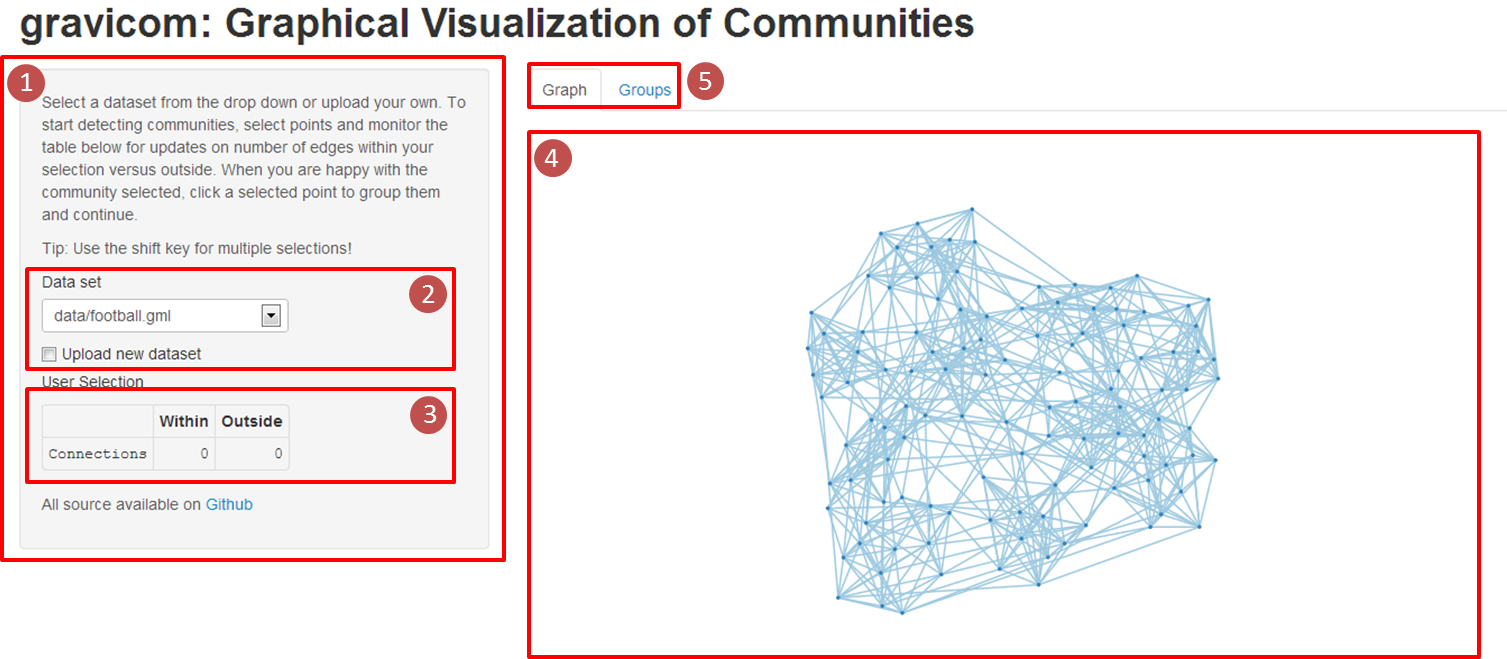
\includegraphics[width=\textwidth]{images/sitecomponents.png}
\caption{\label{fig:sitecomponents} The components that make up gravicom, (1) Control panel, (2) Data management, (3) Connection table, (4) Graph display, and (5) Tabset.}
\end{figure}

Each of these pieces serves as a means for the user to interact with gravicom, either through controls that allow user input to gravicom or through direct interaction with diagnostics and visualization of a graph. Their placement on the gravicom interface can be seen in figure~\ref{fig:sitecomponents}.

\paragraph{Control Panel}
The control panel serves as the starting point for a user's session in gravicom. It contains intructions for the user, as well as the means for a user to select a dataset and the diagnostic connection table. Additionally, the control panel contains a link to the source code for gravicom, should a user be interested in the inner workings of gravicom.

\paragraph{Data Management}
The data management piece is made up of two main parts, data selection and data download. The data selection can be accomplished in two ways, the first being a drop down to select pre-loaded datasets to display. Currently there are two toy datasets in gravicom, a college football dataset and a karate friends dataset. From the dropdown the user can change the dataset to display in the graph. The second part of data selection gives the user the ability to upload his own dataset. Upon clicking the ``Upload new dataset" checkbox, a file selection control appears which gives the user the ability to upload his own graph data to explore with gravicom. This is shown in figure~\ref{fig:uploadnewdataset}. 

\begin{figure}[H]
\centering

\includegraphics[]{images/uploadnewdataset.png}
\caption{\label{fig:uploadnewdataset} The data selection area upon clicking the ``Upload new dataset" checkbox.}
\end{figure}

Data can be downloaded from gravicom with current communities stored. This feature can be used as a save point in working with a graph or as a means to export changes made in gravicom to another tool.



\paragraph{Connection Table}
The connection table is a diagnostic tool for the user to help determine if he has detected a community in his graph. The  table displays the number of connections within a user's selection of nodes in the graph and the number of connections from nodes in a user's selection to nodes not in the selection. The comparison of these two numbers can give the user an idea of if what he has selected is a community or not. The idea behind the connection table is that a community will have more connections within than connections to nodes outside the community.  To aid in the comparison, there is also a proportion column that displays the ratio of number of connections within a selection to the number of connections outside the selection. 

\paragraph{Graph Display}
The graph display shows an interactive graphical representation of  the selected (or uploaded) graph data. Upon load, the graph displays all nodes and edges in the dataset using a force-directed layout algorithm. The user has several ways to interact with the graph: drag, select, and group. A user can drag a node at any time. % to attempt to get a better view of potential communities. However, the graph is setup with a gravity parameter that generally keeps the graph in the center of the screen. 
Upon dragging, the force-directed layout is  rerun, giving an altered view of the graph. Figure~\ref{fig:graphdrag} shows a graph in the process of being dragged.

\begin{figure}[H]
\centering
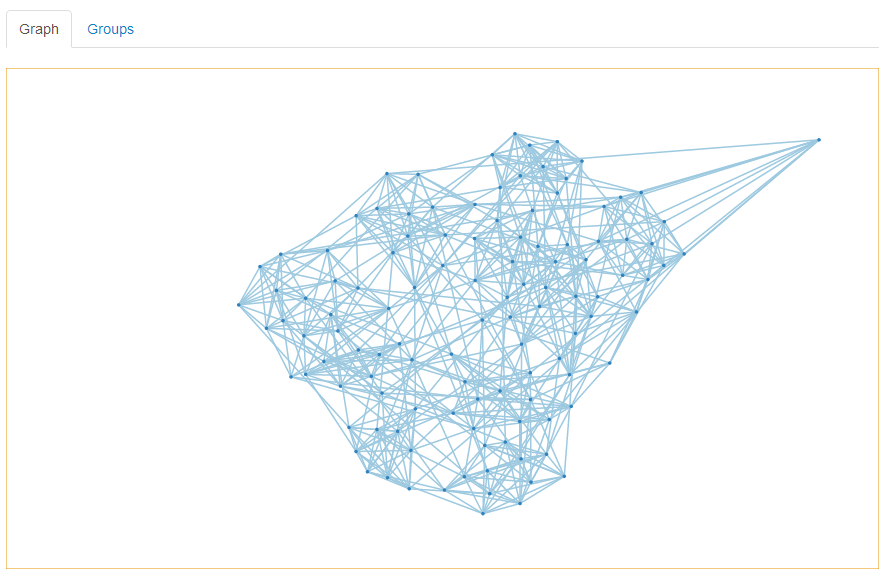
\includegraphics[width=\textwidth]{images/graphdrag.png}
\caption{\label{fig:graphdrag} A graph in the process of being dragged. \hh{Would it be possible to put some marker on the node that's being dragged?}}
\end{figure}

Selection and grouping of  nodes are actions working together: in order to group nodes, a user  first selects a community based on a visual appraisal of the graph. To select nodes the user clicks and drags a selection box around nodes. See figure~\ref{fig:graphselect} for the results of selection in the interface. The shift key can also be used for multiple selections. Upon selection, the connection table is updated and the user can evaluate their selection as a community and alter the selection if need be (the shift key selection is very useful in this step).

\begin{figure}[H]
\centering
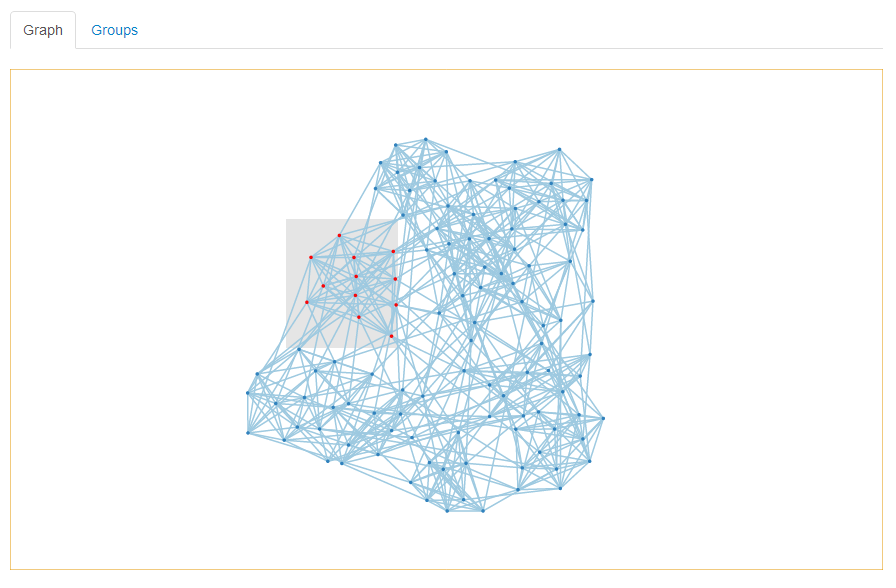
\includegraphics[width=\textwidth]{images/graphselect.png}
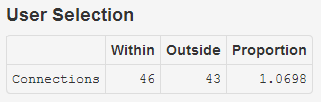
\includegraphics[]{images/tableselect.png}
\caption{\label{fig:graphselect} A graph in the process of nodes being selected. Upon selection of nodes, the connection table updates to display within and outside edges.}
\end{figure}

Selected nodes can be grouped together. Once grouped, a new node is created that comprises all grouped nodes and grouped within edges in size and charge. The force-directed layout is again run, showing the new graph with nodes grouped. This is shown in figure~\ref{fig:graphgroup}. Additionally, grouped nodes are ungrouped by clicking on a grouped node. This process can be repeated until all nodes have been grouped or the user is satisfied that all communities have been detected. 

\begin{figure}[H]
\centering
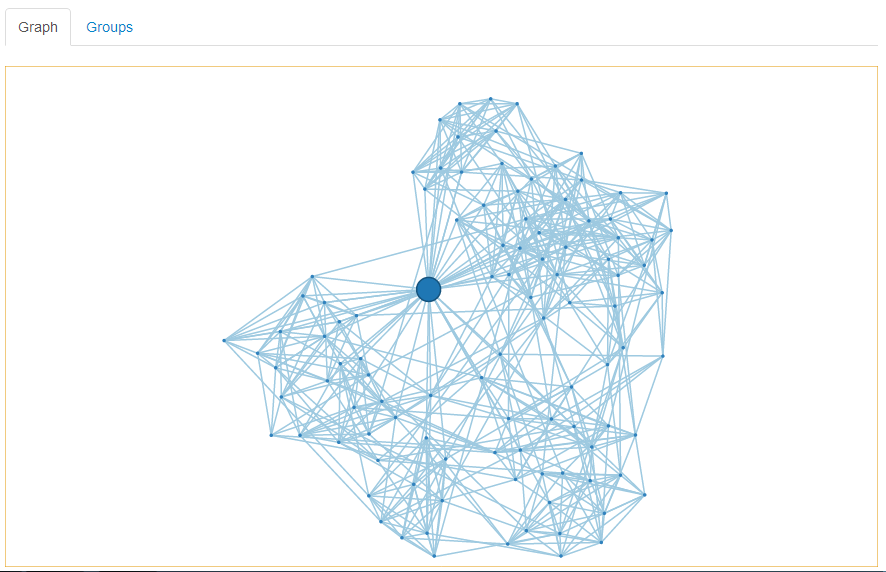
\includegraphics[width=\textwidth]{images/graphgroup.png}
\caption{\label{fig:graphgroup} A graph after nodes have been grouped and the force-directed algorithm has been re-run.}
\end{figure}

\paragraph{Tabset}
The tabset allows the user to switch between two tabs on the screen. The first (and default tab) shows the graph display. The second tab shows the groups that a user has created in the graph. Each group show how many nodes are contained in that group as well as the ability to drop down and view the nodes contained in that group. If the data are equipped with node labels, these will be displayed. If there are no node labels provided, node IDs will be shown. For an example, see figure~\ref{fig:groupstab}.

\begin{figure}[H]
\centering
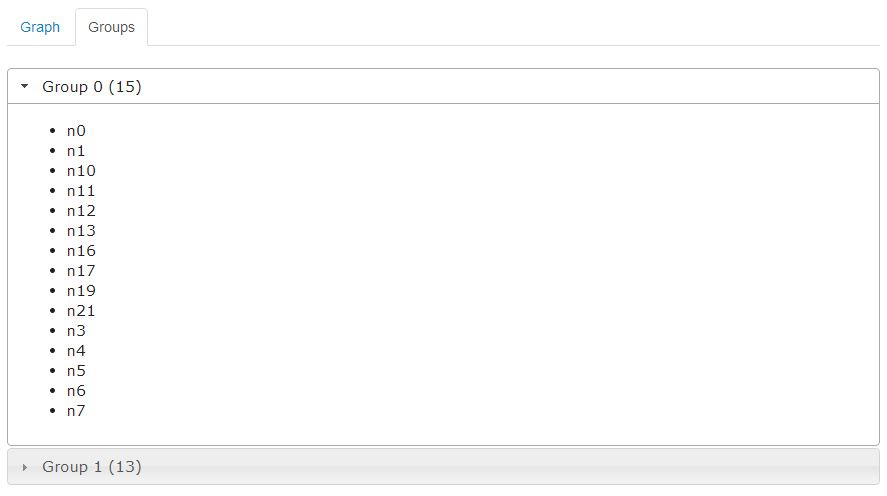
\includegraphics[width=\textwidth]{images/groupstab.png}
\caption{\label{fig:groupstab} The groups tabset displaying which nodes have been grouped in Group 0, for example. The groups tabset also shows that Group 0 has 15 nodes, while Group 1 has 13 nodes.}
\end{figure}


\subsection{Examples}

To demonstrate the use of gravicom, we present three real-world network datasets and explore their community structure.

\subsubsection{College Football}
The first dataset is a representation of U.S. College Football Division 1 games from the 2000 season \cite{gn-football}. In this network, nodes represent teams and an edge represents a regular-season game played between the two teams connected. The network as it looks on load in gravicom is presented in figure~\ref{fig:football_1}. 
\hh{You should say that the distances between the nodes are based on the number of games played between the teams.}

\begin{figure}[H]
\centering
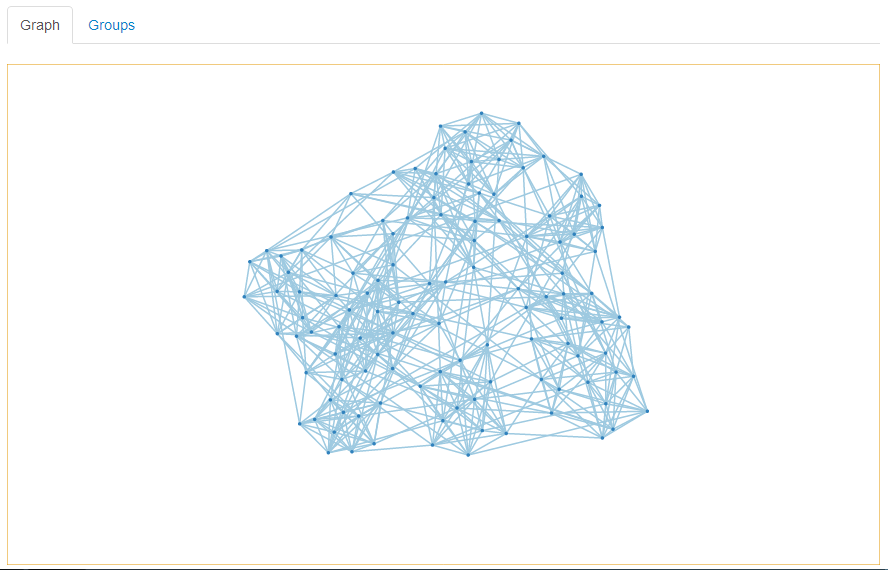
\includegraphics[width=\textwidth]{images/football_1.png}
\caption{\label{fig:football_1} College Football network represented in gravicom. \hh{What do you want the user to see? Pick one aspect.}}
\end{figure}

Colleges within the same football conference will play members of their conference more frequently than teams outside of their conference, making this an interesting dataset to try to detect communities in. This is also an ideal example due to the relatively small number of nodes and edges present, making a graphical representation feasible. One challenge encountered with this dataset is that there are independent teams like Notre Dame that are not in a conference, and so may complicate community detection. Another complication is that small conference schools will typically play large conference schools in the beginning of the season in order to pay for their athletic programs, which could cause there to be more edges than expected between small conferences and large conferences.

Upon viewing the network in gravicom, some likely communities emerge and by selecting nodes to determine within and outside edges, we can classify colleges into conferences, as seen in figure~\ref{fig:football_2}.

\begin{figure}[H]
\centering
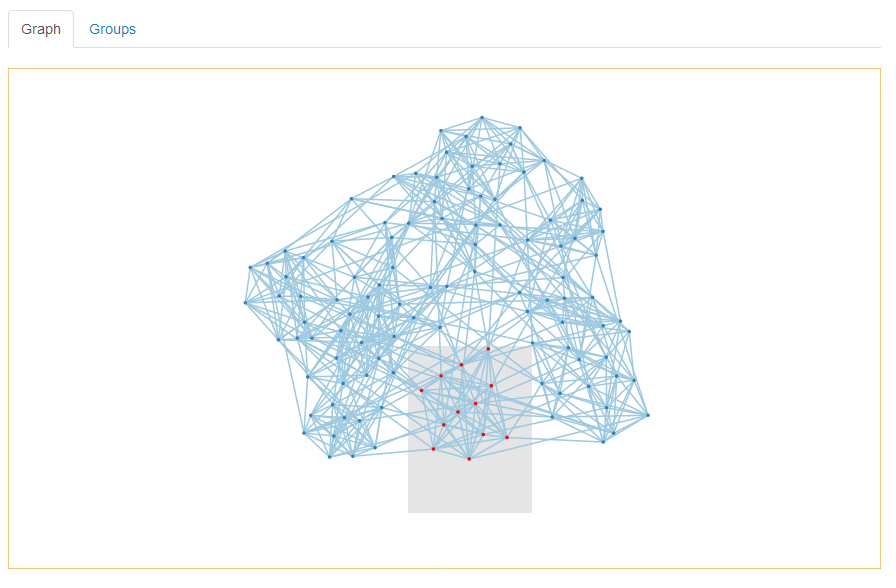
\includegraphics[width=\textwidth]{images/football_2.png}
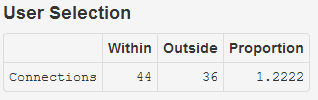
\includegraphics[]{images/football_3.png}
\caption{\label{fig:football_2} Selecting a potential community in gravicom and assessing the number of within verses outside selection edges.}
\end{figure}

Once the user is satisfied that he has selected a viable community, he clicks to group those nodes and the graph will update to reflect this, allowing new communities to potentially become more easily apparent as seen in figure~\ref{fig:football_4}. 

\begin{figure}[H]
\centering
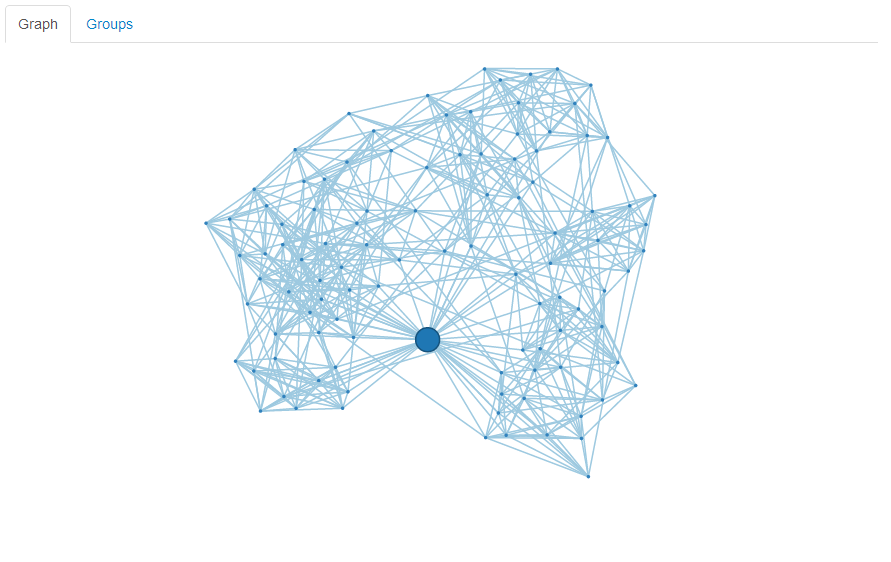
\includegraphics[width=\textwidth]{images/football_4.png}
\caption{\label{fig:football_4} After the first community is detected, more communities become apparent in the network.}
\end{figure}

Additionally, the user can check which nodes were grouped in each community. In this example (figure~\ref{fig:football_5}), we can see the first community detected roughly corresponds to the Big 10, with independent Notre Dame being grouped in the Big 10 due to playing two Big 10 teams in 2000.

\begin{figure}[H]
\centering

\includegraphics[width=\textwidth]{images/football_5.png}
\caption{\label{fig:football_5} A drill-down of the first grouped community which roughly corresponds to the Big 10 Conference.}
\end{figure}

After the first community has been selected, another community at the top of the graph has been revealed. The user can once again, select and group this community and take a look at the nodes in the community as seen in figure~\ref{fig:football_6}. The second conference grouped corresponds exactly to the SEC Conference, another large college football conference. The first two communities to become evident correspond to large Division 1 conferences that play the majority of their games within conference, matching our earlier assertion that small conferences would be more difficult to detect.

\begin{figure}[H]
\centering
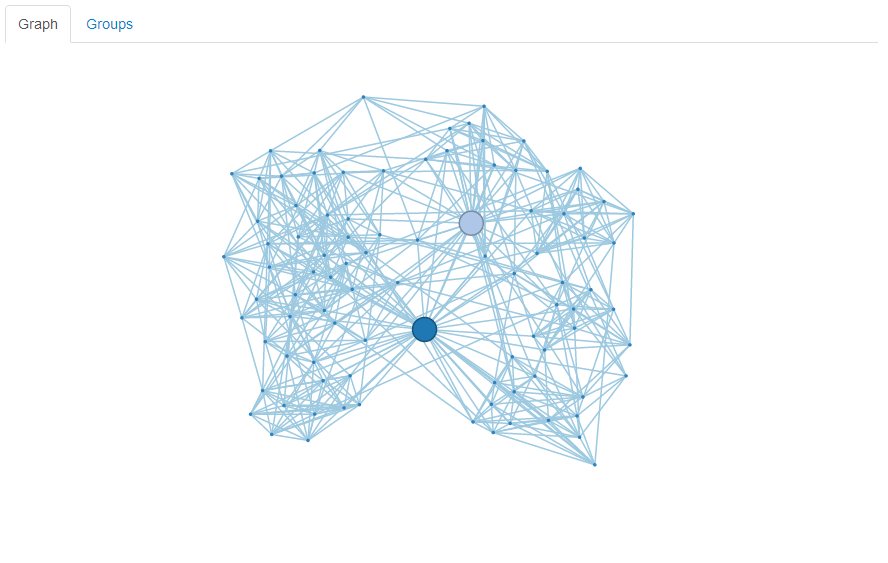
\includegraphics[width=\textwidth]{images/football_6.png}

\includegraphics[width=\textwidth]{images/football_7.png}
\caption{\label{fig:football_6} A second community is grouped which corresponds to the SEC Conference.}
\end{figure}




This process can be repeated until the user is satisfied with the communities selected. The conclusion of this process is seen in figure~\ref{fig:football_8}. We detected visually 11 conferences in the dataset. There were 11 conferences and 5 independent schools in the dataset. Through manual specification of conferences, we were able to correctly classify 91.3\% of the football teams into their conferences.

\begin{figure}[H]
\centering
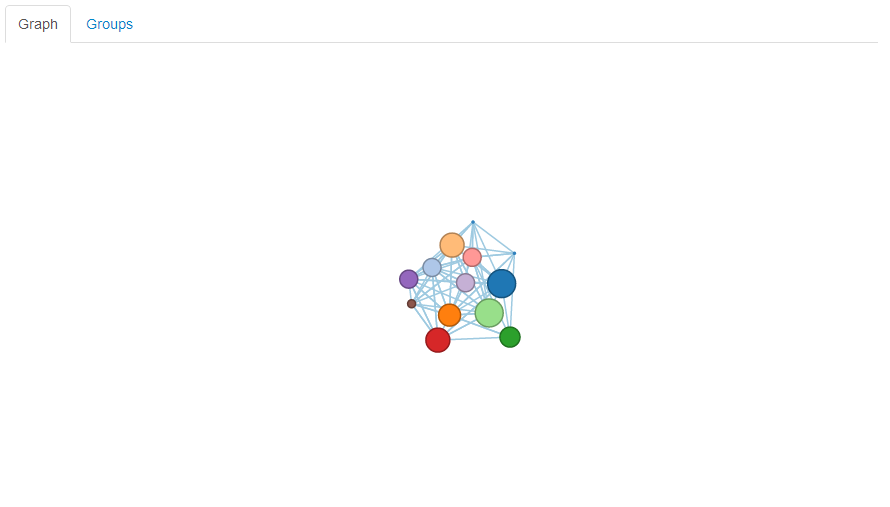
\includegraphics[width=\textwidth]{images/football_8.png}
\caption{\label{fig:football_8} Final community structure detected in gravicom.}
\end{figure}

\subsubsection{Political Books Sold}
The second example dataset is a network of political books published close to the 2004 United States presidential election and sold on Amazon.com \cite{polbooks}. Each node represents a book and each edge represents frequent copurchasing of two books by the same buyers. The books are classified as being conservative, liberal, or neutral in the data set and we can see a clear partition in figure~\ref{fig:polbooks_1} between two main groups with a smaller group between as a connection when looking at the network in gravicom. This dataset is interesting because it highlights a great divide in the United States population that can be ascribed to the two party political system. 

\begin{figure}[H]
\centering
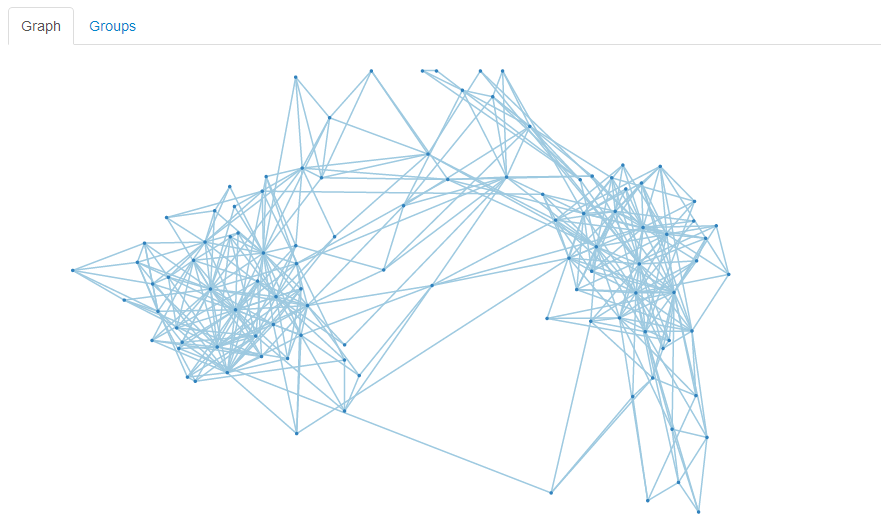
\includegraphics[width=\textwidth]{images/polbooks_1.png}
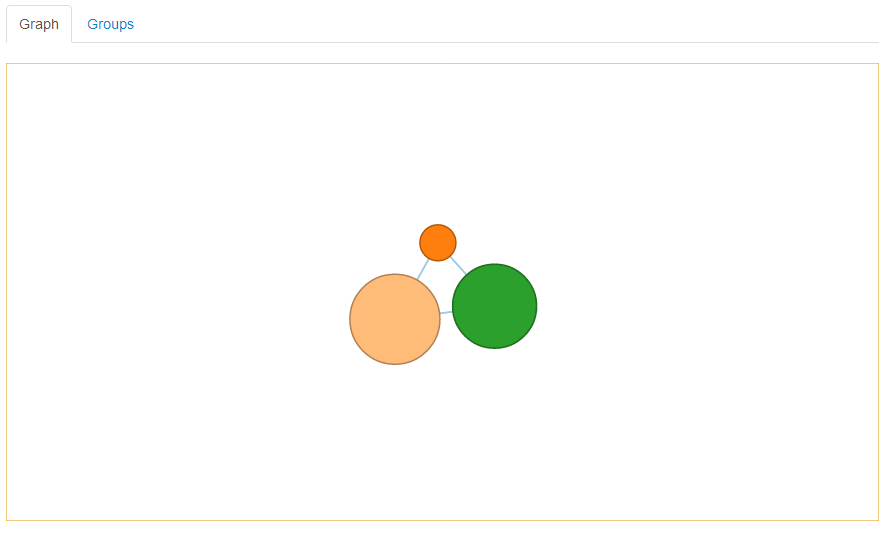
\includegraphics[width=\textwidth]{images/polbooks_2.png}
\caption{\label{fig:polbooks_1} Political books dataset as seen in gravicom prior and post community detection.}
\end{figure}



We detected visually 3 types of books in the dataset. Through manual specification of types of books, we were able to correctly classify 86.67\% of the books into their categories. \hh{What is `correct' based on?}
%output of above xtable
% latex table generated in R 3.0.2 by xtable 1.7-1 package
% Wed Nov 06 18:32:14 2013
% \begin{table}[ht]
% \centering
% \begin{tabular}{llllll}
% \hline
% \multicolumn{2}{c}{gravicom Liberal} & \multicolumn{2}{c}{gravicom Conservative} & \multicolumn{2}{c}{gravicom gravicom Neutral} \\
%   \hline
%   \hline
% Book Title & Actual Category & Book Title & Actual Category & Book Title & Actual Category \\ 
%   \hline
% Bush at War & Conservative & A National Party No More & Conservative & Bush vs. the Beltway & Conservative \\ 
%   Downsize This! & Liberal & Dereliction of Duty & Conservative & Charlie Wilson's War & Conservative \\ 
%   The Culture of Fear & Liberal & Ten Minutes from Normal & Conservative & Dangerous Dimplomacy & Conservative \\ 
%   House of Bush, House of Saud & Liberal & Bush Country & Conservative & The Man Who Warned America & Conservative \\ 
%   The Best Democracy Money Can Buy & Liberal & Rumsfeld's War & Conservative & Rise of the Vulcans & Conservative \\ 
%   Rogue Nation & Liberal & Legacy & Conservative & Allies & Conservative \\ 
%   Stupid White Men & Liberal & Hating America & Conservative & Soft Power & Liberal \\ 
%   Rush Limbaugh Is a Big Fat Idiot & Liberal & Hillary's Scheme & Conservative & The Choice & Liberal \\ 
%   The Great Unraveling & Liberal & Let Freedom Ring & Conservative & America Unbound & Liberal \\ 
%   Against All Enemies & Liberal & Tales from the Left Coast & Conservative & 1000 Years for Revenge & Neutral \\ 
%   American Dynasty & Liberal & Breakdown & Conservative & Colossus & Neutral \\ 
%   The Price of Loyalty & Liberal & Losing Bin Laden & Conservative & Why America Slept & Neutral \\ 
%   The Sorrows of Empire & Liberal & The French Betrayal of America & Conservative & Ghost Wars & Neutral \\ 
%   Worse Than Watergate & Liberal & Spin Sisters & Conservative & Sleeping With the Devil & Neutral \\ 
%   Perfectly Legal & Liberal & The Right Man & Conservative & Empire & Neutral \\ 
%   Big Lies & Liberal & Useful Idiots & Conservative & The Future of Freedom & Neutral \\ 
%   The Lies of George W. Bush & Liberal & Shut Up and Sing & Conservative & All the Shah's Men & Neutral \\ 
%   Bushwomen & Liberal & Who's Looking Out for You? & Conservative & Surprise, Security, the American Experience & Neutral \\ 
%   The Bubble of American Supremacy & Liberal & Those Who Trespass & Conservative &   &   \\ 
%   Living History & Liberal & Bias & Conservative &   &   \\ 
%   The Politics of Truth & Liberal & The O'Reilly Factor & Conservative &   &   \\ 
%   Fanatics and Fools & Liberal & Persecution & Conservative &   &   \\ 
%   Bushwhacked & Liberal & Deliver Us from Evil & Conservative &   &   \\ 
%   Disarming Iraq & Liberal & Give Me a Break & Conservative &   &   \\ 
%   Lies and the Lying Liars Who Tell Them & Liberal & Betrayal & Conservative &   &   \\ 
%   MoveOn's 50 Ways to Love Your Country & Liberal & The Real America & Conservative &   &   \\ 
%   The Buying of the President 2004 & Liberal & The Faith of George W Bush & Conservative &   &   \\ 
%   Buck Up Suck Up & Liberal & The Death of Right and Wrong & Conservative &   &   \\ 
%   Hegemony or Survival & Liberal & The Third Terrorist & Conservative &   &   \\ 
%   The New Pearl Harbor & Liberal & Arrogance & Conservative &   &   \\ 
%   Freethinkers & Liberal & The Savage Nation & Conservative &   &   \\ 
%   Had Enough? & Liberal & The Bushes & Conservative &   &   \\ 
%   It's Still the Economy, Stupid! & Liberal & Things Worth Fighting For & Conservative &   &   \\ 
%   We're Right They're Wrong & Liberal & Off with Their Heads & Conservative &   &   \\ 
%   What Liberal Media? & Liberal & We Will Prevail & Conservative &   &   \\ 
%   The Clinton Wars & Liberal & Why Courage Matters & Conservative &   &   \\ 
%   Weapons of Mass Deception & Liberal & Hollywood Interrupted & Conservative &   &   \\ 
%   Dude, Where's My Country? & Liberal & The Enemy Within & Conservative &   &   \\ 
%   Thieves in High Places & Liberal & Slander & Conservative &   &   \\ 
%   Shrub & Liberal & Endgame & Conservative &   &   \\ 
%   The Exception to the Rulers & Liberal & The Official Handbook Vast Right Wing Conspiracy & Conservative &   &   \\ 
%   Plan of Attack & Neutral & Fighting Back & Conservative &   &   \\ 
%     &   & Power Plays & Neutral &   &   \\ 
%     &   & Meant To Be & Neutral &   &   \\ 
%     &   & The Perfect Wife & Neutral &   &   \\ 
%    \hline
% \end{tabular}
% \end{table}


\subsection{Technical Aspects}

gravicom utilizes three main pieces of software to establish interactive user control of a random graph as sketched out in figure~\ref{fig:clientserver}. The three pieces used are Shiny, D3, and igraph. They are used to manage server/client interaction, user interface and graph layout, and data formatting, respectively.

\begin{figure}[H]
\centering
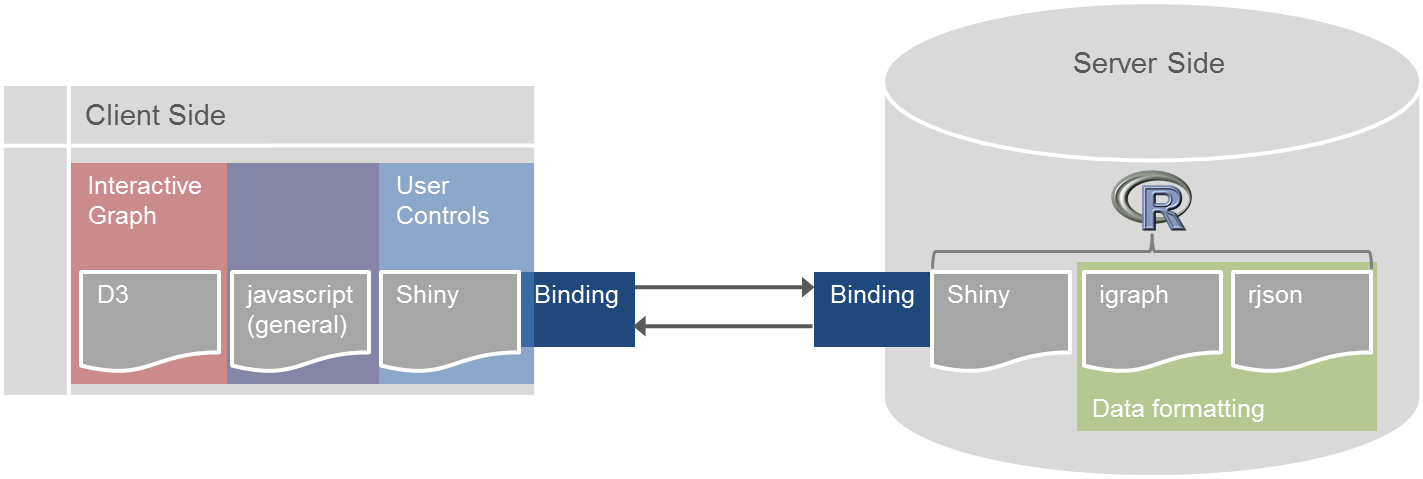
\includegraphics[width=\textwidth]{images/clientserverflow.png}
\caption{\label{fig:clientserver} Relationship between client and server, specifically focusing on how data travels between the two.}
\end{figure}

There are very minimal software requirements for a user of gravicom. The client simply needs to have a JavaScript enabled internet browser with HTML5 compatibility, something which almost any modern browser fulfills (an exception is IE8 and below). 

The server side requirements are more extensive, but this does not affect the user of gravicom, only those wanting to host their own instance of the application. To host gravicom, a Linux server is required, with the following installed:

\begin{itemize}
\item Node.js (0.8.16 or later)
\item {\tt R} (2.15 or later)
\item Shiny {\tt R} package, installed into the machine-wide site library. 
\item Shiny Server
\end{itemize}


\subsubsection{Shiny}

Shiny \cite{rs-shiny} is an {\tt R} package created by RStudio that enables {\tt R} users to create an interactive web application that utilizes {\tt R} as the background engine. Through default methods to build user interface elements in HTML and a handle to the server side code, Shiny is a very simple way to turn {\tt R} code into a website. 

gravicom uses the Shiny functionality to create user controls, pass correctly formatted data to the client, and as a means to display summary information regarding the user's interactions with a graph at any point in time. In this context, Shiny serves as the translator between the formatted data and what the user sees and interacts with on their screen.


\subsubsection{D3}

D3 \cite{mb-d3} stands for ``Data Driven Documents" and is a JavaScript library developed and maintained by Mike Bostock with the  purpose of visualizing and interacting with data in a web-based interface. It is freely available from \url{http://www.d3js.org}. The library facilitates manipulation of HTML elements, SVG (scalable vector graphics), and CSS (cascading style sheets) with the end goal of rendering animations and providing user interactions that are tied to the underlying data. The key idea behind the library is that Document Object Model elements are completely determined by the data. The Document Object Model (DOM) is a convention for representing and interacting with objects in HTML, XHTML and XML. So, rather than adding elements to a web page to be viewed by users, D3 allows users to see and interact with graphical representations of their data in a web framework. 

gravicom uses D3 to handle all graphical displays and user interactions with the graph. The data is passed to the client and able to be used through Shiny's input bindings. It is crucial that the data has been formatted correctly at this point for the JavaScript to properly function. For this reason, we limit the file types being passed in to the tool to a robust graph-specific type.

At this point in the page lifecycle, the graph's nodes are tied to circles and the edges are tied to paths on the page. User manipulations such as selecting, dragging, and grouping are handled by D3 and  data is passed back to the server via Shiny's output bindings to allow for communication between user and the {\tt R} engine underneath. This is illustrated in figure~\ref{fig:pagelifecycle}. What this means is that all visualization and user interaction with the graph are accomplished using JavaScript, more specifically the library D3. Shiny and {\tt R} serve as the framework on which the data sits, but when the user touches the data they are doing so through the JavaScript elements. 

\begin{figure}[H]
\centering
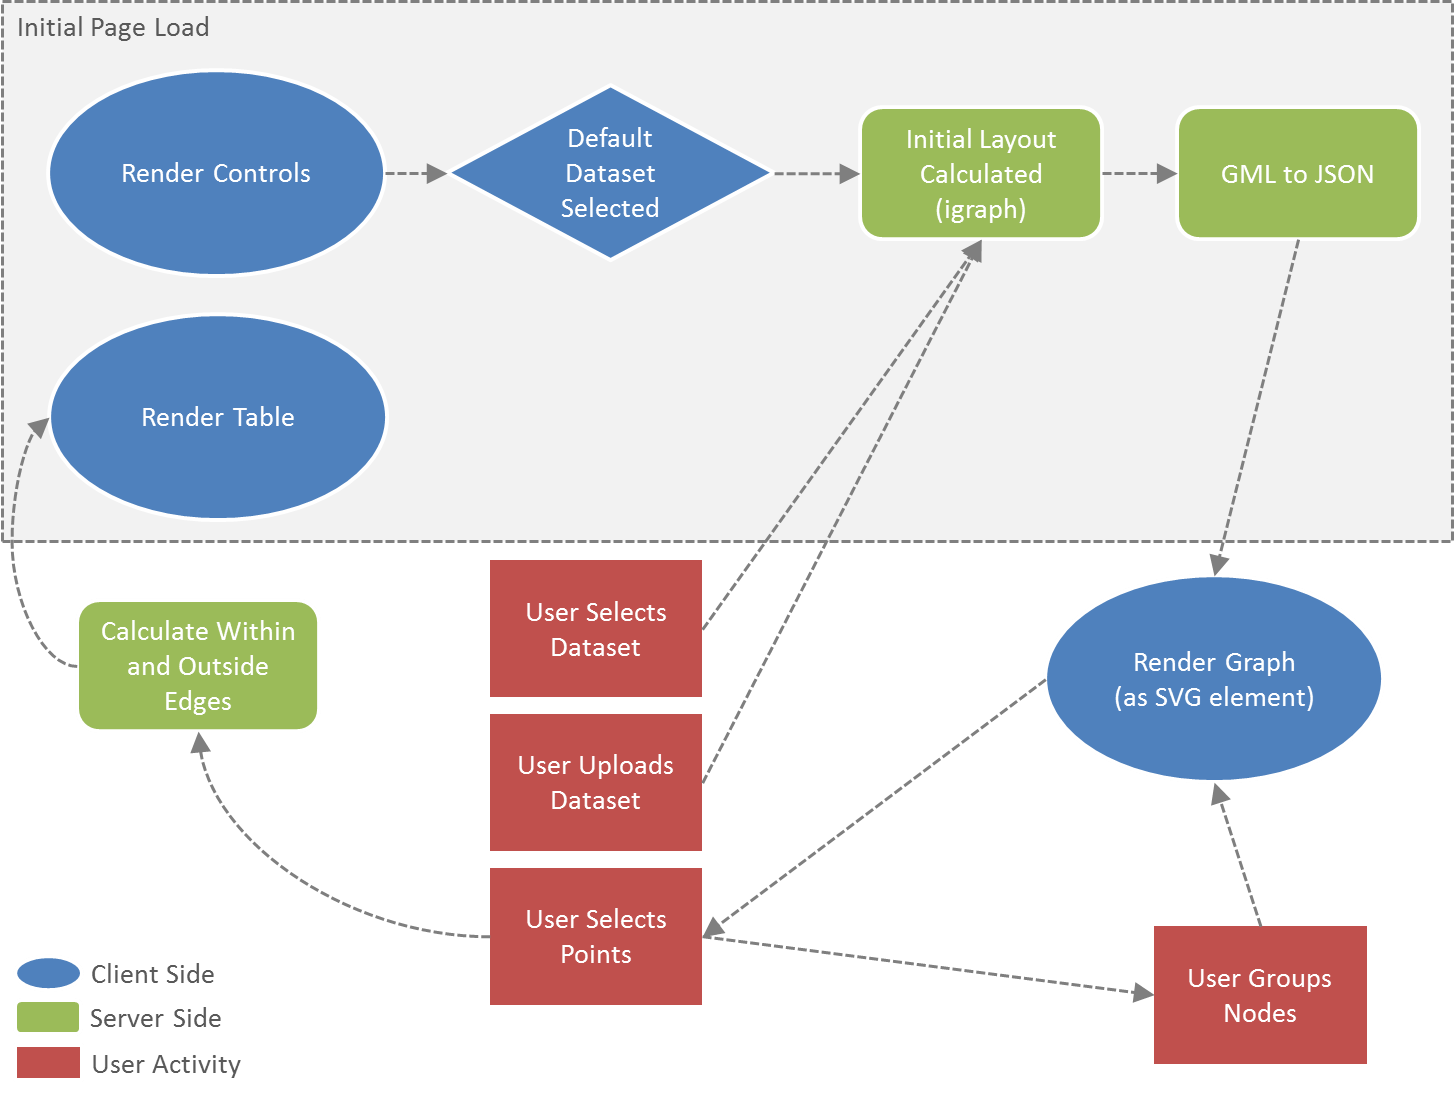
\includegraphics[width=\textwidth]{images/pagelifecycle.png}
\caption{\label{fig:pagelifecycle} Page lifecycle beginning from on load. User actions are highlighted in red, server actions in green, and actions completed on the client side are highlighted in blue.}
\end{figure}


\subsubsection{igraph}

igraph \cite{gc-igraph} is a software package used for creating and manipulating undirected and directed graphs. It is a cross-language package available for C, R, python, and Ruby. igraph also supports multiple graph file formats and visualization of graph structures.

gravicom utilizes two parts of igraph, first is the conversion from a gml file to an XML file. The gml file format, short for Graph Modelling Language, is a hierarchical ASCII-based file format for describing graphs. Below is an example gml file of an undirected graph consisting of two nodes linked by a single edge. The important points to note are that  node identifiers (id) have to be numeric. An edge consists only of source and target ids of the nodes it connects, while  nodes can have other attributes, e.g.~{\tt value} in the example. For a directed graph, the parameter {\tt directed} has to be set to 1, which will result in the edge information on target and source being evaluated accordingly.
\begin{knitrout}
\definecolor{shadecolor}{rgb}{0.969, 0.969, 0.969}\color{fgcolor}\begin{kframe}
\begin{verbatim}
## graph
## [
##   directed 0
##   node
##   [
##     id 0
##     label "Node 1"
##     value 100
##   ]
##   node
##   [
##     id 1
##     label "Node 2"
##     value 200
##   ]
##   edge
##   [
##     source 1
##     target 0
##   ]
## ]
\end{verbatim}
\end{kframe}
\end{knitrout}

For the conversion from an  XML file  to a JSON file we make user of the R package {\tt rjson} \cite{acb-rjson}.  JSON is the native data format used in D3, which  makes working with data in the D3 library incredibly straightforward. Here is our example in the finalized JSON format:
\begin{knitrout}
\definecolor{shadecolor}{rgb}{0.969, 0.969, 0.969}\color{fgcolor}\begin{kframe}
\begin{verbatim}
## {
##   "nodes":
##   [{"id":"n0","v_id":"0","v_label":"Node 1","v_value":"100"}, 
##    {"id":"n1","v_id":"1","v_label":"Node 2","v_value":"200"}], 
##  "edges":
##   [{"source":0, "target":1}]
## }
\end{verbatim}
\end{kframe}
\end{knitrout}

Our example data will yield the graph in figure~\ref{fig:samplegraph}.

\begin{figure}[H]
\centering
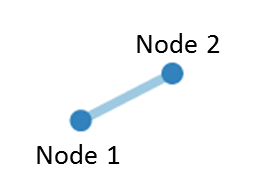
\includegraphics{images/samplegraph.png}
\caption{\label{fig:samplegraph} Graph created from sample gml file.}
\end{figure}
The second use of igraph within gravicom is to compute initial $x$ and $y$ coordinates for the nodes of the graph using a force-driven layout. This provides the initialization for the force-layout algorithm in D3. This reduces the computational load on the clients' side and helps minimize unnecessary movement by the nodes. This is critical as the extra movement at the loading of the pages creates an unnecessarily chaotic start to the user's experience. 




\section{Further Work}

\printbibliography
\end{document}
